
% \begin{figure*}
% \centering
% % 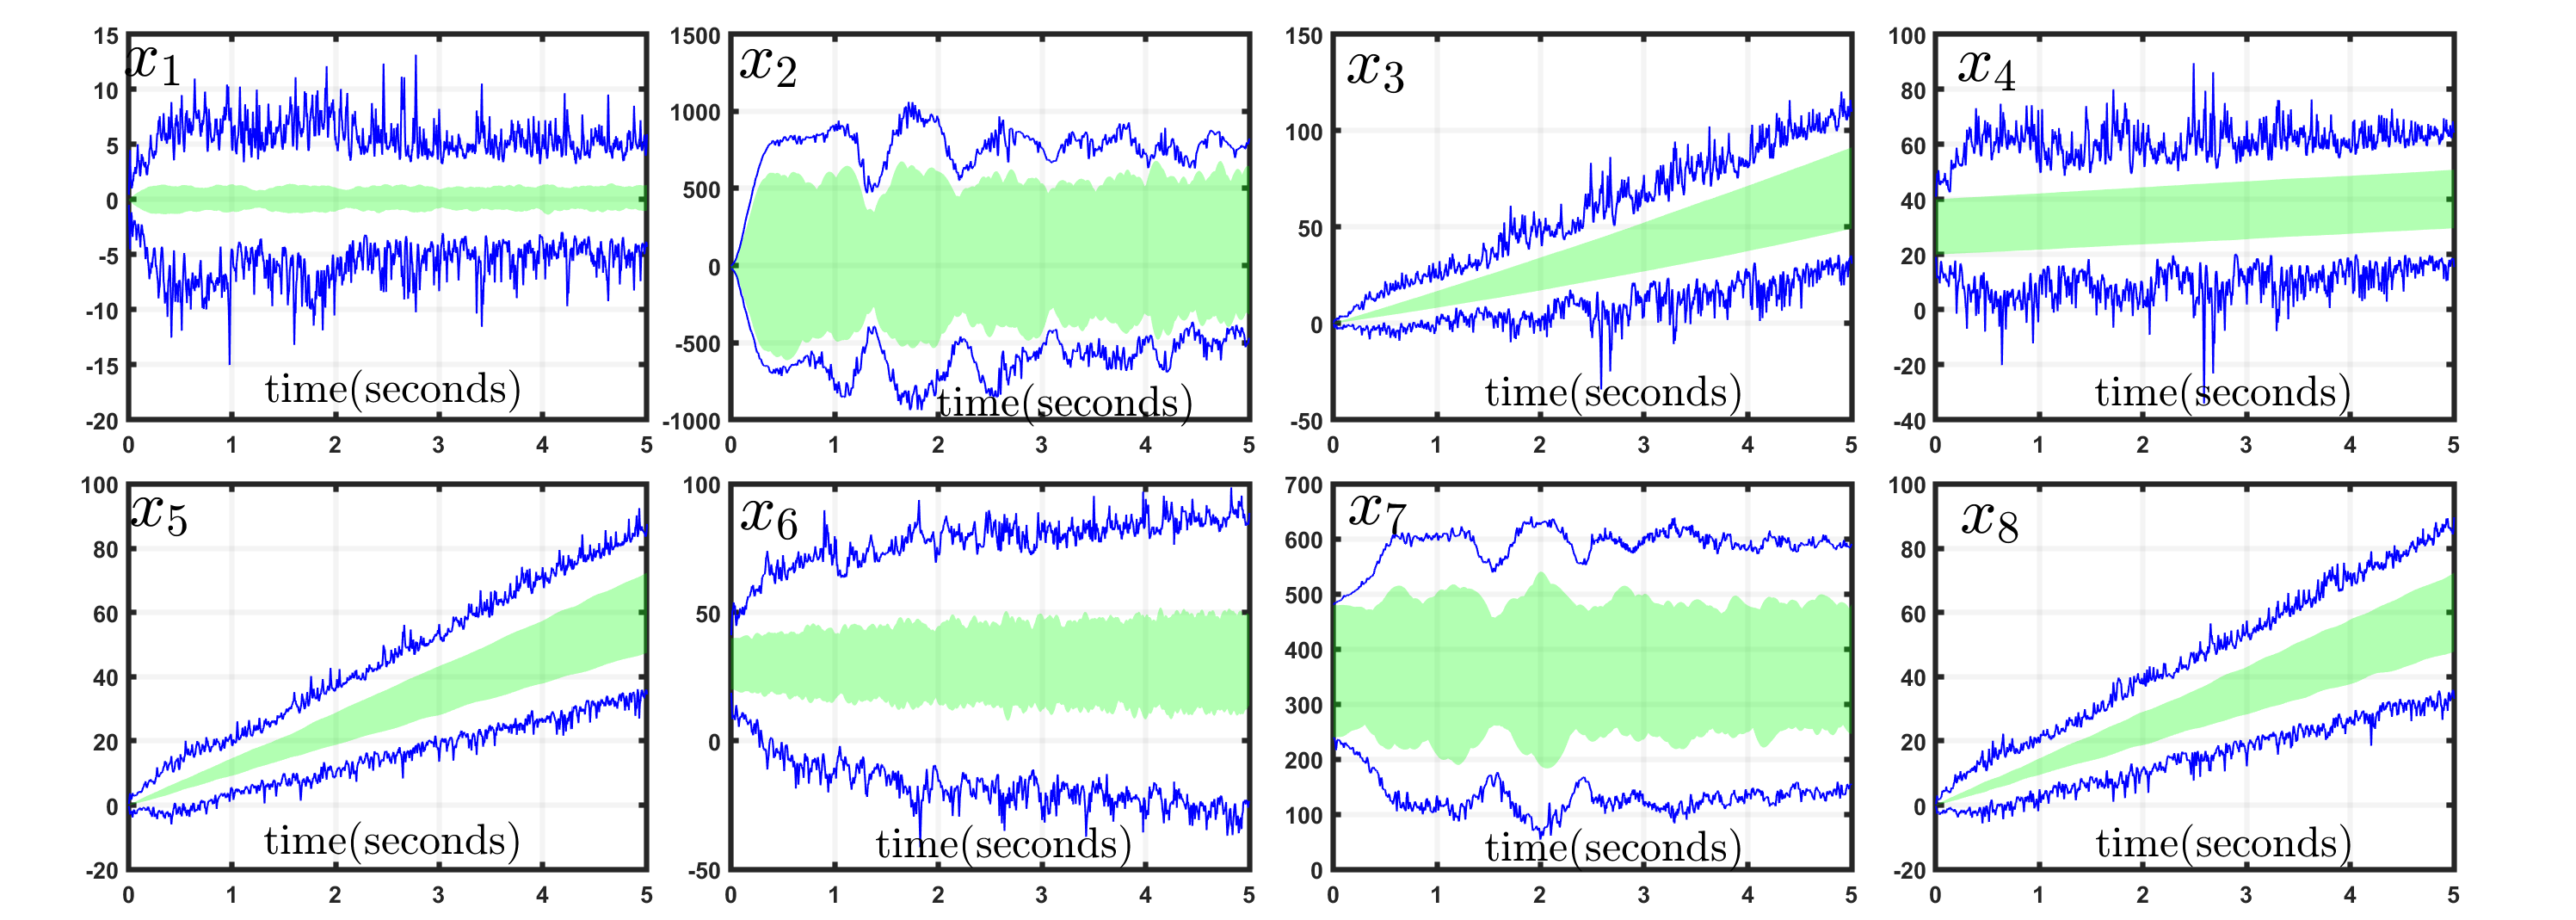
\includegraphics[trim={3.2cm
% %   2cm 3.4cm 2cm},width =\linewidth]{figures/First_8_states2.pdf}
% 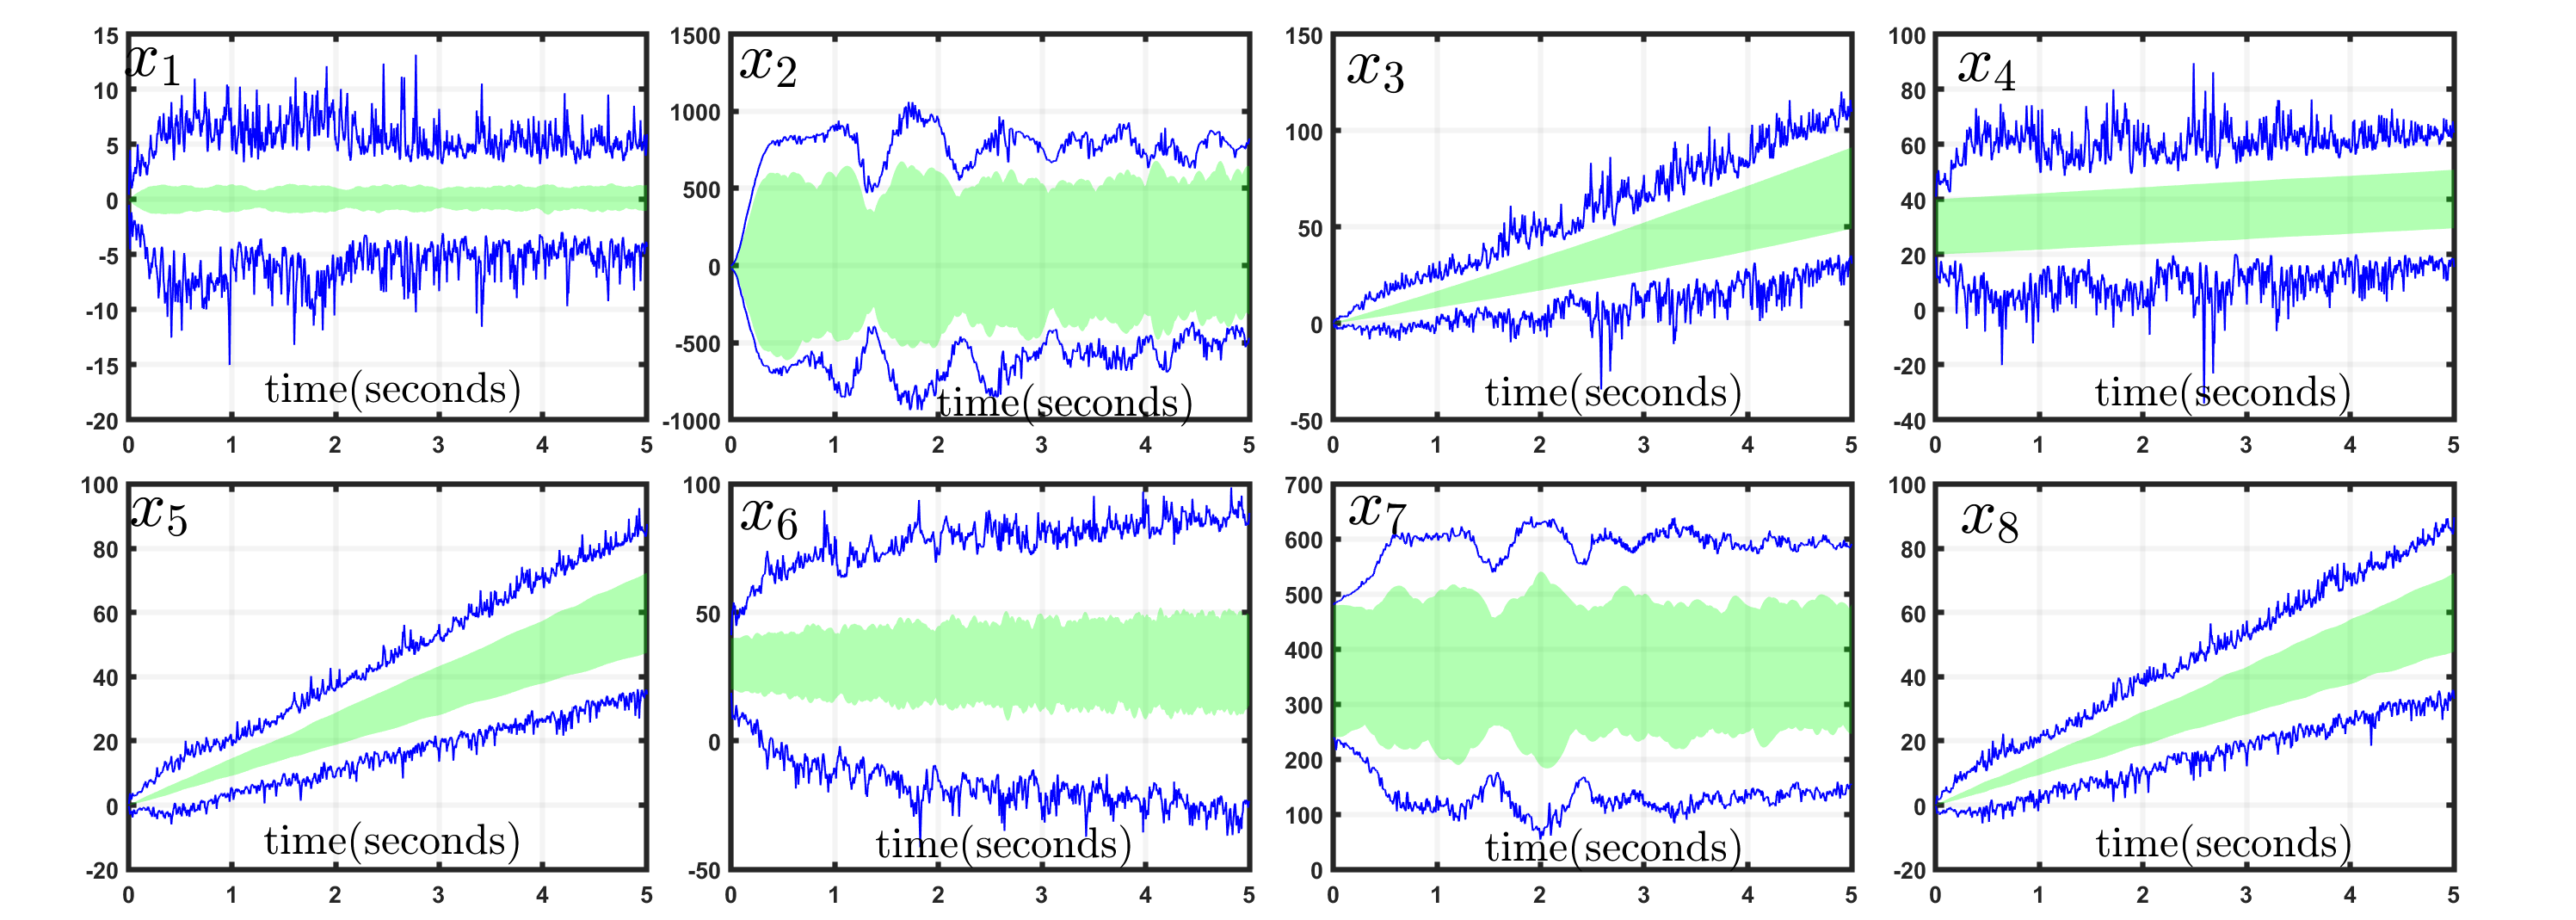
\includegraphics[width =0.7\linewidth]{figures/First_8_states2.pdf}
% \caption{Shows the projection of our $\delta$-confident flowpipe on the first $8$ components of the trajectory state. There is a shift between the distribution of deployment and training environments. The shaded area are the trajectories sampled from the deployment environment.}
% \label{fig:proj}
% \end{figure*}
To simulate real-world systems capable of producing actual trajectory data, we employ stochastic difference equation-based models with additive Gaussian noise to account for uncertainties in observations, dynamics, and potential modeling errors. Our theoretical guarantees apply to any real-world distribution $\trajreal_{\statee_0} \in \dist$, provided that the residual distribution shift $\tv(\distzeroR, \distR)$ is below a given threshold $\tau$. Here we evaluate our results on three different case studies. The first two experiments involve a $12$-D quadcopter with $\tau = 0$, while the final experiment focuses on a $27$-D powertrain model where the distribution shift is upper-bounded at $\tau = 4\%$. In Experiment 1, we compare our approach with \cite{hashemi2024statistical}. However, since that methodology does not scale well for trajectories with large number of time-steps, $\horizon$, we address Experiments 2 and 3, only using the methodology proposed in this paper. The next two sections provide a general overview of the experiments, with detailed information deferred to the Appendix. Table \ref{tbl:expdetails} also presents the details of the numerical results.

% To demonstrate the tightness of our $\delta$-confident flowpipe, we empirically examine it by sampling i.i.d. trajectories from an arbitrary real-world distribution $\dist$ such that $\tilde{\tau}<\tau$,\footnote{We use a worst-case scenario where $\tilde{\tau}$ is close to $\tau$.} and calculating the ratio of trajectories that fall within the probabilistic flowpipes. We denote this ratio as $\tilde{\delta}$.

% In the following, we analyze a $12$-dimensional stochastic system for a quadcopter and initially compare our results with those in \cite{hashemi2024statistical} to demonstrate improved accuracy. To illustrate enhanced scalability, we conduct another case study on the quadcopter with significantly longer trajectories. Finally, we perform reachability on a $27$-dimensional hybrid system known as the powertrain, as proposed in \cite{althoff2012avoiding}. However, since this model is deterministic, we add Gaussian system noise into the proposed dynamics before collecting the training and calibration datasets.
% \begin{table*}
% \centering
% \begin{tabular*}{\linewidth}{@{\extracolsep{\fill}}cccccccccc}
% \cmidrule{1-10}
% \muc{1}{} & \muc{2}{Specification} & \muc{3}{Training} & \muc{2}{Surrogate Reachability} & \muc{2}{Inflating Hypercube}\\
% \cmidrule{2-3}\cmidrule{4-6}\cmidrule{7-8} \cmidrule{9-10}
% Exp $\#$: & $\delta$ & $\tau$ & $\#$ & avg runtime & $\mid \traindataset \mid$ & $\#$ & avg runtime (method) & runtime & $\mid \calibdataset \mid$ \\
% \cmidrule{1-10}
% 1 & $99.99\%$ & $0$ & $100$ & $39.6\ \sec$ & $42,000$ & $100$ & $1.43\ \sec\ $ (E) & $2.08\ \sec$ & $20,000$ \\
% 2 & $99.99\%$ & $0$ & $451$ & $33.65\ \sec$ & $20,000$ & $4501$ & $0.030\ \sec\ $ (E) & $116.58\ \sec$ & $20,000$ \\
% 3 & $95\%$ & $4\%$ & $400$ & $40.6\ \sec$ & $10,000$ & $4000$ & $0.064\ \sec\ $ (A) & $142.02\ \sec$ & $10,000$ \\
% \cmidrule{1-10}
% \end{tabular*}
% \vspace{-3mm}
% \caption{Details of the experiments. Models are trained in parallel using $18$ CPU workers. Training time may vary with the number of workers. E and A denote exact-star and approx-star, respectively.}
% \vspace{-6mm}
% \label{tbl:expdetails}
% \end{table*}
\begin{table*}
\hspace{1mm}
\resizebox{0.85\textwidth}{!}{
\begin{tabular*}{\textwidth}{@{\extracolsep{\fill}}cccccccccc}
\cmidrule{1-10}
\muc{1}{} & \muc{2}{Specification} & \muc{3}{Training} & \muc{2}{Surrogate Reachability} & \muc{2}{Inflating Hypercube}\\
\cmidrule{2-3}\cmidrule{4-6}\cmidrule{7-8} \cmidrule{9-10}
    Exp $\#$: & $\delta$ & $\tau$  & $\#$ & avg runtime  & $\mid \traindataset \mid$  &  $\#$ & avg runtime(method)  & runtime & $\mid \calibdataset \mid$  \\
\cmidrule{1-10}
1    & $99.99\%$   & $0$    & $100$ & $39.6\ \sec$  &  $42,000$ & $100$  & $1.43\ \sec\ $ (E)   & $2.08\ \sec$ & $20,000$\\
2    & $99.99\%$   & $0$    & $451$ & $33.65\ \sec$  &  $20,000$ & $4501$ & $0.030\ \sec\ $ (E)  & $116.58\ \sec$ & $20,000$\\
3    & $95\%$      & $4\%$  & $400$ & $40.6\ \sec$  &  $10,000$ & $4000$ & $0.064\ \sec\ $ (A)  & $142.02\ \sec$ & $10,000$\\
\cmidrule{1-10}
\end{tabular*}
}
\vspace{-3mm}\\
\caption{Shows details of the experiments. The models are trained in parallel with $18$ CPU workers. Thus, the average training runtime may vary by selecting different number of workers. The words E, and A represent exact-star and approx-star, respectively.  }
\vspace{-6mm}
\label{tbl:expdetails}
\end{table*}
\vspace{-2mm}
\subsection{$12$-Dimensional Quadcopter}
\vspace{-2mm}
We consider the $12$-dimensional quadcopter system under stochastic conditions for two different case studies. Trajectories are simulated using two ODE models from \cite{hashemi2024statistical} and \cite{hashemi2024scaling} as our simulators. The state variables include the quadcopter's position $(x_1, x_2, x_3)$, velocity $(x_4, x_5, x_6)$, Euler angles $(x_7, x_8, x_9)$ representing roll, pitch, and yaw angles, and angular velocities $(x_{10}, x_{11}, x_{12})$. We also include zero mean additive Gaussian process noise $v \sim \gaussian(0_{12\times1}, \Sigma_v)$ to the simulators with covariance $\Sigma_v = \mathbf{diag}\left( [0.05 \times \vec{1}_{1\times6} ,\  0.01\times \vec{1}_{1\times6]}]^2 \right)$.  In both examples, the set of initial states $\statee_0 \in \init$ is taken from the cited papers, with the distribution $\statee_0 \sim \mathcal{W}$ being uniform.
\vspace{-2mm}
\subsection{27-Dimensional Powertrain }
\vspace{-2mm}
We use the powertrain system proposed by \cite{althoff2012avoiding} as our simulator, which is a hybrid system with three modes. To introduce stochastic conditions, we add zero-mean Gaussian process noise, $v \sim \gaussian(\vec{0}_{27\times1}, \Sigma_v)$, where $\Sigma_v = \mathbf{diag}\left( 10^{-5}\times \vec{1}_{1\times27} \right)$, to their simulator, defining the distribution $\trajsim_{\statee_0}\sim \distzero$.
% For a system with $\beta$ rotating masses, the model follows a $2\beta + 7$ dimensional ODE; in this case, we assume $\beta=10$. 
This system is highly sensitive to noise, which is a key reason we addressed it in this paper. For example, Figure \ref{fig:noisecontribution} shows the angular velocity of the last rotating mass, $x_{27}$, both with and without noise. Following \cite{althoff2012avoiding}, we simulate trajectories with a sampling time of $\delta t = 0.0005$ over a horizon of $2$ seconds ($\horizon = 4000$), and consider their set of initial states $\init$ \footnote{In this case the set $\init$ proposed in \cite{althoff2012avoiding} is a large and high dimensional set, thus the exact star does not scale, and we are restricted to utilized approx star for surrogate reachability.}. We also define the trajectory division setting as $N=4000$, $T_q=1, q\in[N]$. The $\relu$ NN models are with structure $[27, 54,27]$. To reduce the training runtime, we again follow the analytical interpolation strategy we introduced for Experiment 2.

